\PassOptionsToPackage{table}{xcolor}
\documentclass[aspectratio=169,10pt]{beamer}

\usetheme{Madrid}
\usecolortheme{seahorse}
\setbeamertemplate{navigation symbols}{}
\setbeamertemplate{footline}[frame number]

\usepackage{booktabs}
\usepackage{amsmath}
\usepackage{graphicx}
\usepackage{colortbl}
\usepackage{tikz}
\usetikzlibrary{arrows.meta, positioning, shapes.geometric, calc}

% Custom colors
\definecolor{umblue}{RGB}{0,39,76}
\definecolor{ummaize}{RGB}{255,203,5}
\definecolor{todocolor}{RGB}{220,50,50}
\definecolor{lightgray}{RGB}{240,240,240}
\definecolor{gpuA40}{RGB}{70,130,180}
\definecolor{gpuA100}{RGB}{60,179,113}
\definecolor{gpuH100}{RGB}{255,140,0}
\definecolor{gpuV100}{RGB}{169,169,169}
\definecolor{gpuL40S}{RGB}{148,103,189}

\setbeamercolor{title}{fg=umblue}
\setbeamercolor{frametitle}{fg=umblue}

\newcommand{\todo}[1]{\textcolor{todocolor}{\textbf{[TODO: #1]}}}

\title[cp.async Cross-GPU Study]{Predicting \texttt{cp.async} Pipeline Effectiveness\\from Memory-Subsystem Parameters:\\A Cross-GPU Study}
\author{Xiangchen Song \quad Chenxin Geng \quad Yuyang Feng \quad Tian Xia}
\institute{EECS 570 -- Parallel Computer Architecture \\ University of Michigan}
\date{Milestone 1 \quad March 20, 2026}

\begin{document}

% ============================================================
% Slide 1: Title
% ============================================================
\begin{frame}
\titlepage
\end{frame}

% ============================================================
% Slide 2: Problem & Motivation
% ============================================================
\begin{frame}{Problem \& Motivation}

\begin{columns}[T]
\begin{column}{0.55\textwidth}
\textbf{Background:}
\begin{itemize}
    \item NVIDIA \texttt{cp.async} (Ampere+) enables asynchronous global$\to$shared memory copies, overlapping with computation
    \item CUTLASS, FlashAttention-3, Triton all rely on multi-stage \texttt{cp.async} pipelines; pipeline depth $S$ is a key tuning knob
\end{itemize}

\vspace{0.5em}
\textbf{The Problem:}
\begin{itemize}
    \item Practitioners tune $S$ on \emph{one} GPU and assume it transfers
    \item But pipeline effectiveness depends on \textbf{L2 capacity}, \textbf{memory BW/latency}, and \textbf{per-SM shared memory} --- which vary \emph{dramatically} across GPUs
    \item No existing autotuner uses architecture parameters to prune the search space
\end{itemize}
\end{column}

\begin{column}{0.42\textwidth}
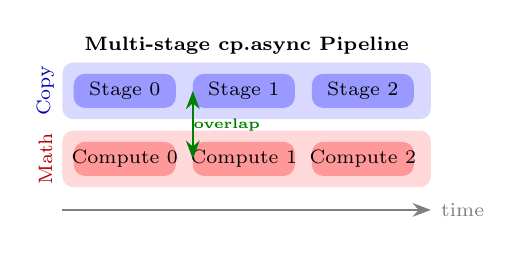
\begin{tikzpicture}[scale=0.72, every node/.style={font=\scriptsize}]
    % cp.async pipeline diagram
    \fill[blue!15, rounded corners] (0,3.2) rectangle (6.5,4.2);
    \fill[red!15, rounded corners]  (0,2.0) rectangle (6.5,3.0);

    \node[font=\scriptsize\bfseries] at (3.25,4.5) {Multi-stage cp.async Pipeline};

    % Stage labels
    \foreach \i/\label in {0/Stage 0, 1/Stage 1, 2/Stage 2} {
        \fill[blue!40, rounded corners] (0.2+\i*2.1, 3.4) rectangle (2.0+\i*2.1, 4.0);
        \node at (1.1+\i*2.1, 3.7) {\label};
    }
    \foreach \i/\label in {0/Compute 0, 1/Compute 1, 2/Compute 2} {
        \fill[red!40, rounded corners] (0.2+\i*2.1, 2.2) rectangle (2.0+\i*2.1, 2.8);
        \node at (1.1+\i*2.1, 2.5) {\label};
    }

    \node[font=\scriptsize, blue!70!black] at (-0.3, 3.7) [rotate=90] {Copy};
    \node[font=\scriptsize, red!70!black]  at (-0.3, 2.5) [rotate=90] {Math};

    \draw[-{Stealth}, thick, gray] (0,1.6) -- (6.5,1.6) node[right] {time};

    % Overlap arrow
    \draw[{Stealth}-{Stealth}, thick, green!50!black] (2.3,2.5) -- (2.3,3.7);
    \node[green!50!black, font=\tiny\bfseries] at (2.9,3.1) {overlap};
\end{tikzpicture}

\vspace{0.3em}
\begin{block}{\small Research Question}
\scriptsize Does optimal $S^*$ and its speedup diverge across GPUs with different memory subsystems? Can a parameter-free model predict this?
\end{block}
\end{column}
\end{columns}
\end{frame}

% ============================================================
% Slide 3: Hypotheses
% ============================================================
\begin{frame}{Three Falsifiable Hypotheses}

\begin{description}\small
    \item[H1 -- L2-capacity driven:] Speedup inflects when working set $W_{\text{conc}} > C_{\text{L2}}$. \\
    \textcolor{gray}{\scriptsize Test: L40S (96\,MB nominal / 99\,MB measured) should see minimal benefit; A40 (6\,MB nominal / 8\,MB measured) should see largest benefit at large $N$.}

    \vspace{0.5em}
    \item[H2 -- Ridge-point driven:] Low ridge-point GPUs benefit most from pipelining. \\
    \textcolor{gray}{\scriptsize Test: Speedup ordering A100-MIG ($R{=}7.9$) $>$ H100 ($R{=}20$) $>$ A40 ($R{=}53.7$).}

    \vspace{0.5em}
    \item[H3 -- Latency--occupancy tension:] Optimal depth $S^*$ balances DRAM latency hiding vs.\ SMEM-induced occupancy loss. \\
    \textcolor{gray}{\scriptsize Test: $S^*(N)$ non-monotonic on A40 (high latency + small SMEM); flat on H100.}
\end{description}

\vspace{0.8em}
\centering
\small In practice, a \textbf{mixture} is likely --- the predictive model incorporates all three.

\end{frame}

% ============================================================
% Slide 4: Hardware Setup
% ============================================================
\begin{frame}{Experimental Setup: Hardware}

\begin{columns}[T]
\begin{column}{0.58\textwidth}
\renewcommand{\arraystretch}{1.15}
\begin{table}
\centering
\scriptsize
\begin{tabular}{@{}lccccc@{}}
\toprule
 & \textcolor{gpuV100}{\textbf{V100}} & \textcolor{gpuA40}{\textbf{A40}} & \textcolor{gpuA100}{\textbf{A100 MIG}} & \textcolor{gpuL40S}{\textbf{L40S}} & \textcolor{gpuH100}{\textbf{H100}} \\
\midrule
Arch       & Volta  & Ampere & Ampere    & Ada    & Hopper \\
SMs        & 80     & 84     & 42        & 142    & 132 \\
\texttt{cp.async} & ---  & \checkmark & \checkmark & \checkmark & \checkmark \\
Memory     & HBM2   & GDDR6  & HBM2e     & GDDR6  & HBM3 \\
Peak BW    & 900    & 696    & 968       & 864    & 3350\,GB/s \\
L2 (nominal) & 6\,MB  & 6\,MB  & 20\,MB & 96\,MB & 50\,MB \\
L2 (measured) & 8\,MB  & 8\,MB  & 24\,MB       & 99\,MB & 28\,MB \\
SMEM/SM    & 96\,KB & 100\,KB & 164\,KB  & 100\,KB & 228\,KB \\
FP32 peak  & 15.7   & 37.4   & 7.6       & 45.7   & 67\,TF \\
\textbf{Ridge}  & 17.4   & \textbf{53.7}  & \textbf{7.9} & 52.9 & 20.0 \\
\midrule
Role & Boundary & \multicolumn{2}{c}{Core contrast} & L2 extreme & Core anchor \\
\bottomrule
\end{tabular}
\end{table}
\end{column}

\begin{column}{0.40\textwidth}
\textbf{Design rationale:}
\begin{itemize}\scriptsize
    \item \textbf{A40 vs H100}: max memory-subsystem gap ($8.3\times$ L2, $4.8\times$ BW)
    \item \textbf{A100 MIG}: lowest ridge (7.9), measured L2 = 24\,MB $\to$ H2 predicts most benefit; tests MIG
    \item \textbf{L40S}: largest L2 (96\,MB nominal, 99\,MB measured) $\to$ tests ``L2 absorbs all'' extreme
    \item \textbf{V100}: no \texttt{cp.async} $\to$ boundary condition ($1.0\times$)
\end{itemize}

\vspace{0.3em}
\scriptsize
\textbf{Key finding:} Measured L2 $\neq$ nominal on all GPUs. V100/A40: 6$\to$8\,MB; A100-MIG: 20$\to$24\,MB; L40S: 96$\to$99\,MB; H100: 50$\to$28\,MB (L2 slicing).
\end{column}
\end{columns}
\end{frame}

% ============================================================
% Slide 5: Kernels & Methodology
% ============================================================
\begin{frame}{Experimental Setup: Kernels \& Methodology}

\begin{columns}[T]
\begin{column}{0.50\textwidth}
\textbf{Two complementary kernel families:}

\vspace{0.3em}
\renewcommand{\arraystretch}{1.2}
\begin{table}
\centering
\scriptsize
\begin{tabular}{@{}llp{3.5cm}@{}}
\toprule
\textbf{ID} & \textbf{GPUs} & \textbf{Description} \\
\midrule
V0-GEMM & All & Naive global load, no tiling \\
V1-GEMM & All & Shared-mem tiling, sync load \\
V3-GEMM & A40+ & \texttt{cp.async} pipeline, $S \in \{2,3,4\}$ \\
\midrule
V1-Stencil & All & 1D stencil, sync shared-mem \\
V3-Stencil & A40+ & \texttt{cp.async} pipelined, $S \in \{2,3,4\}$ \\
\midrule
Ref & All & cuBLAS SGEMM (ceiling) \\
\bottomrule
\end{tabular}
\end{table}

\vspace{0.3em}
\scriptsize
Same V3 source code runs on A40, A100-MIG, H100 --- \textbf{no GPU-specific branches}.
\end{column}

\begin{column}{0.48\textwidth}
\textbf{Why these two kernels?}
\begin{itemize}\scriptsize
    \item \textbf{GEMM}: compute-bound ($\text{AI} \gg R$) but still has per-tile memory stalls
    \item \textbf{Stencil}: memory-bound ($\text{AI} \approx 5$ FLOP/B), near/below ridge point
    \item If predictor works for both $\to$ captures general memory-subsystem properties
\end{itemize}

\vspace{0.5em}
\textbf{Workload sweep:}
\begin{itemize}\scriptsize
    \item GEMM: $N \in \{256, 512, \ldots, 8192\}$
    \item Tile sizes: $T \in \{16, 32, 64, 128\}$
    \item Stencil: $L \in \{2^{16}, 2^{18}, \ldots, 2^{26}\}$
\end{itemize}

\vspace{0.5em}
\textbf{Measurement:}
\begin{itemize}\scriptsize
    \item \texttt{cudaEvent\_t}, 3 warmup + 10 timed, median
    \item Correctness: cuBLAS (GEMM) / CPU (stencil)
\end{itemize}
\end{column}
\end{columns}
\end{frame}

% ============================================================
% Slide 6: Tools & Predictive Model
% ============================================================
\begin{frame}{Predictive Model (Parameter-Free)}

\begin{columns}[T]
\begin{column}{0.45\textwidth}
\textbf{Idea:} predict \texttt{cp.async} speedup from architecture constants alone (no fitted parameters).

\vspace{0.8em}
\textbf{Three inputs per GPU} (from pointer-chase microbenchmark):
\begin{itemize}\scriptsize
    \item Effective L2 capacity $C_{\text{L2}}^{\text{eff}}$
    \item L2 latency $L_{\text{L2}}$, DRAM latency $L_{\text{DRAM}}$
\end{itemize}

\vspace{0.8em}
\textbf{Key modeling choices:}
\begin{itemize}\scriptsize
    \item \textbf{280-cycle floor} on per-stage compute --- sync + async overhead dominates small tiles
    \item \textbf{$\alpha{=}0.15$} --- occupancy loss is highly sub-linear
\end{itemize}

\vspace{0.8em}
\scriptsize
\textbf{Tools:} CMake + SLURM, Nsight Compute, pointer-chasing microbenchmark
\end{column}

\begin{column}{0.53\textwidth}
\begin{block}{\small Core Formula}
\vspace{-0.3em}
\scriptsize
\begin{align*}
h_{\text{hit}} &= \min\!\bigl(1,\; C_{\text{L2}}^{\text{eff}} \,/\, W_{\text{conc}}\bigr)
    & & \text{\tiny L2 hit fraction} \\[2pt]
L_{\text{eff}} &= h_{\text{hit}} \cdot L_{\text{L2}} + (1{-}h_{\text{hit}}) \cdot L_{\text{DRAM}}
    & & \text{\tiny effective memory latency (cycles)} \\[2pt]
T_{\text{compute}} &= \max\!\bigl(T_{\text{compute}}^{\text{raw}},\; 280\bigr)
    & & \text{\tiny per-stage compute window (cycles)}
\end{align*}
\end{block}

\vspace{0.2em}
\begin{block}{\small Predicted Speedup}
\vspace{-0.5em}
\[
\widehat{S}_{\text{pred}} = \underbrace{\frac{\max(T_{\text{compute}},\; L_{\text{eff}})}{\max\!\bigl(T_{\text{compute}},\; L_{\text{eff}}\,/\,S_{\text{stage}}\bigr)}}_{\text{overlap benefit}} \times \underbrace{\left(\frac{\text{Occ}(S_{\text{stage}})}{\text{Occ}(1)}\right)^{0.15}}_{\text{occupancy penalty}}
\]
\end{block}

\vspace{0.1em}
\scriptsize
\renewcommand{\arraystretch}{1.0}
\begin{tabular}{@{}r@{\;=\;}l@{\qquad}r@{\;=\;}l@{}}
$C_{\text{L2}}^{\text{eff}}$ & effective L2 capacity &
$L_{\text{L2}}$, $L_{\text{DRAM}}$ & L2 / DRAM latency \\
$W_{\text{conc}}$ & concurrent working set &
$S_{\text{stage}}$ & pipeline depth (2,3,4) \\
$T_{\text{compute}}^{\text{raw}}$ & pure FLOP time per stage &
$\text{Occ}(S)$ & blocks per SM at depth $S$ \\
\end{tabular}

\vspace{0.2em}
\centering
\scriptsize
\textbf{All inputs} = arch constants + microbenchmark values.\;
\emph{Zero} parameters fitted from kernel data.
\end{column}
\end{columns}
\end{frame}

% ============================================================
% Slide 7: Results & Key Findings
% ============================================================
\begin{frame}{Results \& Key Findings}

\begin{columns}[T]
\begin{column}{0.36\textwidth}
\textbf{Model Accuracy (MAPE):}

\vspace{0.2em}
\renewcommand{\arraystretch}{1.15}
\begin{table}
\centering
\scriptsize
\begin{tabular}{@{}lcc@{}}
\toprule
\textbf{GPU} & \textbf{GEMM} & \textbf{Stencil} \\
\midrule
\textcolor{gpuV100}{V100}   & \multicolumn{2}{c}{\textit{no cp.async}} \\
\textcolor{gpuA40}{A40}     & 11.1\% & 4.1\% \\
\textcolor{gpuA100}{A100 MIG} & 9.2\% & 6.7\% \\
\textcolor{gpuL40S}{L40S}   & 5.7\% & 7.2\% \\
\textcolor{gpuH100}{H100}   & 9.9\% & 5.5\% \\
\midrule
\textbf{Overall (4 GPUs)} & \textbf{9.0\%} & \textbf{5.9\%} \\
\bottomrule
\end{tabular}
\end{table}

\vspace{0.2em}
\textbf{Measured L2 $\neq$ Nominal:}
\vspace{0.1em}
\renewcommand{\arraystretch}{1.1}
\begin{table}
\centering
\scriptsize
\begin{tabular}{@{}lrr@{}}
\toprule
\textbf{GPU} & \textbf{Nom.} & \textbf{Eff.} \\
\midrule
V100 & 6\,MB  & 8\,MB \\
A40  & 6\,MB  & 8\,MB \\
A100 MIG & 20\,MB & 24\,MB \\
L40S & 96\,MB & 99\,MB \\
H100 & 50\,MB & \textbf{28\,MB} \\
\bottomrule
\end{tabular}
\end{table}
\end{column}

\begin{column}{0.62\textwidth}
\textbf{Hypothesis Status:}
\begin{itemize}\scriptsize
    \item[\textcolor{green!60!black}{\textbf{H1}}] \textbf{Supported.} $W_{\text{conc}}/C_{\text{L2}}$ is primary driver.
    \item[\textcolor{yellow!60!black}{\textbf{H2}}] \textbf{Partial.} Ridge point alone insufficient --- must combine with L2/latency.
    \item[\textcolor{green!60!black}{\textbf{H3}}] \textbf{Supported.} A40 tile=64 stage=3: occupancy drop causes slowdown.
\end{itemize}

\vspace{0.2em}
\textbf{Predicted vs.\ Measured Speedup (GEMM, $N{=}4096$, tile=16):}

\vspace{0.1em}
\renewcommand{\arraystretch}{1.1}
\begin{table}
\centering
\scriptsize
\begin{tabular}{@{}l cc cc cc@{}}
\toprule
 & \multicolumn{2}{c}{\textbf{$S{=}2$}} & \multicolumn{2}{c}{\textbf{$S{=}3$}} & \multicolumn{2}{c}{\textbf{$S{=}4$}} \\
\cmidrule(lr){2-3}\cmidrule(lr){4-5}\cmidrule(lr){6-7}
\textbf{GPU} & Pred & Meas & Pred & Meas & Pred & Meas \\
\midrule
\textcolor{gpuA40}{A40}      & 0.96 & 0.98 & 0.90 & 0.98 & 0.86 & 0.98 \\
\textcolor{gpuA100}{A100}    & 1.00 & 1.00 & 0.98 & 0.99 & 0.93 & 1.00 \\
\textcolor{gpuL40S}{L40S}    & 1.01 & 0.96 & 0.95 & 0.97 & 0.91 & 0.98 \\
\textcolor{gpuH100}{H100}    & 1.03 & 0.92 & 1.03 & 0.88 & 1.03 & 0.91 \\
\bottomrule
\end{tabular}
\end{table}

\vspace{0.1em}
\centering\scriptsize
\textbf{Key insight:} Zero-parameter model correctly identifies $S^*{=}1$ as optimal on 3/4 cp.async GPUs. H100 mismatch reveals Hopper-specific async costs not captured by latency/occupancy alone --- a clear direction for refinement.
\end{column}
\end{columns}
\end{frame}

% ============================================================
% Slide 9: Next Steps & Timeline
% ============================================================
\begin{frame}{Next Steps \& Timeline}

\begin{columns}[T]
\begin{column}{0.55\textwidth}
\renewcommand{\arraystretch}{1.3}
\begin{table}
\centering
\scriptsize
\begin{tabular}{@{}clp{4.5cm}@{}}
\toprule
\textbf{Week} & \textbf{Lead} & \textbf{Milestone} \\
\midrule
\rowcolor{green!10} 1--2 & A+C & \checkmark~Build system, V0/V1 baselines, pointer-chasing microbench \\
\rowcolor{green!10} 3--4 & B & \checkmark~V3-GEMM/Stencil impl, initial A40 curves \\
\rowcolor{green!10} 5--6 & B+D & \checkmark~5-GPU full comparison (V100/A40/A100-MIG/L40S/H100), model validation, \textbf{Milestone 1} \\
\midrule
7--8 & C+D & Nsight anomaly deep-dives, $\bigstar$Triton pre-filter \\
9--10 & All & Pipeline benefit maps, final figures, report + poster \\
\bottomrule
\end{tabular}
\end{table}

\vspace{0.3em}
\scriptsize \colorbox{green!10}{\strut Completed}
\end{column}

\begin{column}{0.43\textwidth}
\textbf{Remaining work (Weeks 7--10):}
\begin{itemize}\scriptsize
    \item Nsight Compute deep-dives on top-5 MAPE outliers
    \item $\bigstar$ Triton pre-filter: measure autotune time reduction and false-negative rate
    \item Pipeline benefit heatmaps (AI $\times$ $W_{\text{conc}}/C_{\text{L2}}$)
    \item Leave-one-out cross-validation across 5 GPUs
    \item Final report (6-page, conference format)
    \item Poster ($30'' \times 40''$)
\end{itemize}

\vspace{0.3em}
\textbf{Key risks:}\\
\scriptsize H100 directional mismatch (pred $>1$, meas $<1$) --- Hopper async overhead not modeled. A100-MIG tile=32 underpredicts by $\sim$13\% --- occupancy model needs MIG refinement.
\end{column}
\end{columns}
\end{frame}

\end{document}
